\section{Case study}\label{sec:caseStudy}
In this section we show the application of the proposed UML bridge to a non-trivial case study.
The objective of this case study is to present how each aspect of the proposed approach works in practice.

\begin{figure}[htbp]
	\centering
		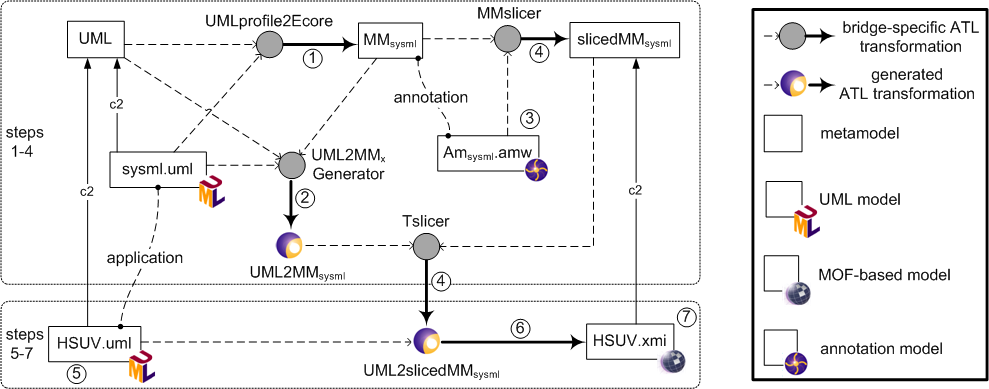
\includegraphics[width=1\textwidth]{figures/caseStudy.png}
	\caption{Overview of the HSUV case study}
	\label{fig:caseStudy}
\end{figure}

As shown in Figure \ref{fig:caseStudy}, we organized the case study as a seven-steps process:
%
\begin{enumerate}
	\item Transformation of the SysML profile into a MOF metamodel called $MM_{sysml}$;
	\item Automatic generation of model-to-model transformations from SysML-profiled models to MOF-based models and vice versa;
	\item Creation of an annotation model $am_{sysml}$ to slice $MM_{sysml}$;
	\item Execution of \textit{MMslicer} and \textit{Tslicer} according to the $am_{sysml}$;
	\item Design of a SysML-profiled UML model ($hsuv.uml$ in figure);
	\item Transformation of $hsuv.uml$ into its MOF-based counterpart ($hsuv.xmi$);
	\item Development of a simple manipulation tool that works on $hsuv.xmi$.
\end{enumerate}
%
Before going into the details of each step, it is important to note that the first four steps are executed only once for each
UML profile to bridge, whereas steps five to seven ...
\ivano{da notare che i punti da 1 a 4 verranno eseguiti una sola volta, mentre gli altri sono eseguiti per ogni modello che vogliamo gestire}

\ivano{introdurre sysml}

\ivano{dire che  metamodello otteniamo}

\ivano{descrivere il modello sysml HSUV, lo abbiamo preso dalla superstructure di UML e modellato in papyrus}

\ivano{descrivere il modello che otteniamo}

\ivano{far vedere un esempietto di trasformazione che simula un tool di manipolazione}

\ivano{paragonarlo con la stessa trasf che avremmo avuto se avessimo dovuto lavorare direttamente con UML}


%The objective of this case study is to present how the UML bridge works at both metamodeling and modeling
%abstraction layers, how the slicing mechanism works in practice, and how a XXX manipulation tool may benefit from
%the application of our approach.